\documentclass{beamer}
\usepackage{graphicx}
\usepackage{amsmath, esint}

\usepackage{ragged2e}
\usepackage{tikz}
\usetikzlibrary{arrows,shapes}

\usepackage{listings}
\lstset{escapeinside={@(}{)@}}
\usepackage{algorithm}
\usepackage{algorithmic}

\usepackage{minted}
\usepackage{xcolor} 
\definecolor{LightGray}{gray}{0.975}

%\usetheme{Warsaw}
\usefonttheme{serif} 

\title[Chapter 3]{Database System Concepts, $7^{th}$ Edition \\ Chapter 3: Introduction to SQL}
\author{Silberschatz, Korth and Sudarshan}
\date{\today}

\setbeamertemplate{navigation symbols}{}%remove navigation symbols

\defbeamertemplate*{footline}{shadow theme}
{%
  \leavevmode%
  \hbox{\begin{beamercolorbox}[wd=.5\paperwidth,ht=2.5ex,dp=1.125ex,leftskip=.3cm plus1fil,rightskip=.3cm]{author in head/foot}%
    \usebeamerfont{author in head/foot} Database System Concepts \hfill \insertshorttitle
  \end{beamercolorbox}%
  \begin{beamercolorbox}[wd=.5\paperwidth,ht=2.5ex,dp=1.125ex,leftskip=.3cm,rightskip=.3cm plus1fil]{title in head/foot}%
    \usebeamerfont{title in head/foot} \hfill \insertframenumber\,/\,\inserttotalframenumber%
  \end{beamercolorbox}}%
  \vskip0pt%
}

\AtBeginSection[]
{
     \begin{frame}<beamer>
     \frametitle{Plan}
     \tableofcontents[currentsection]
     \end{frame}
}

\newcommand{\toRight}[1]{
    \begin{FlushRight}
        {\tiny #1}
    \end{FlushRight}
} % Align to right

\begin{document}

\frame{\titlepage}

\begin{frame}{Database System Concepts}
    \centering
    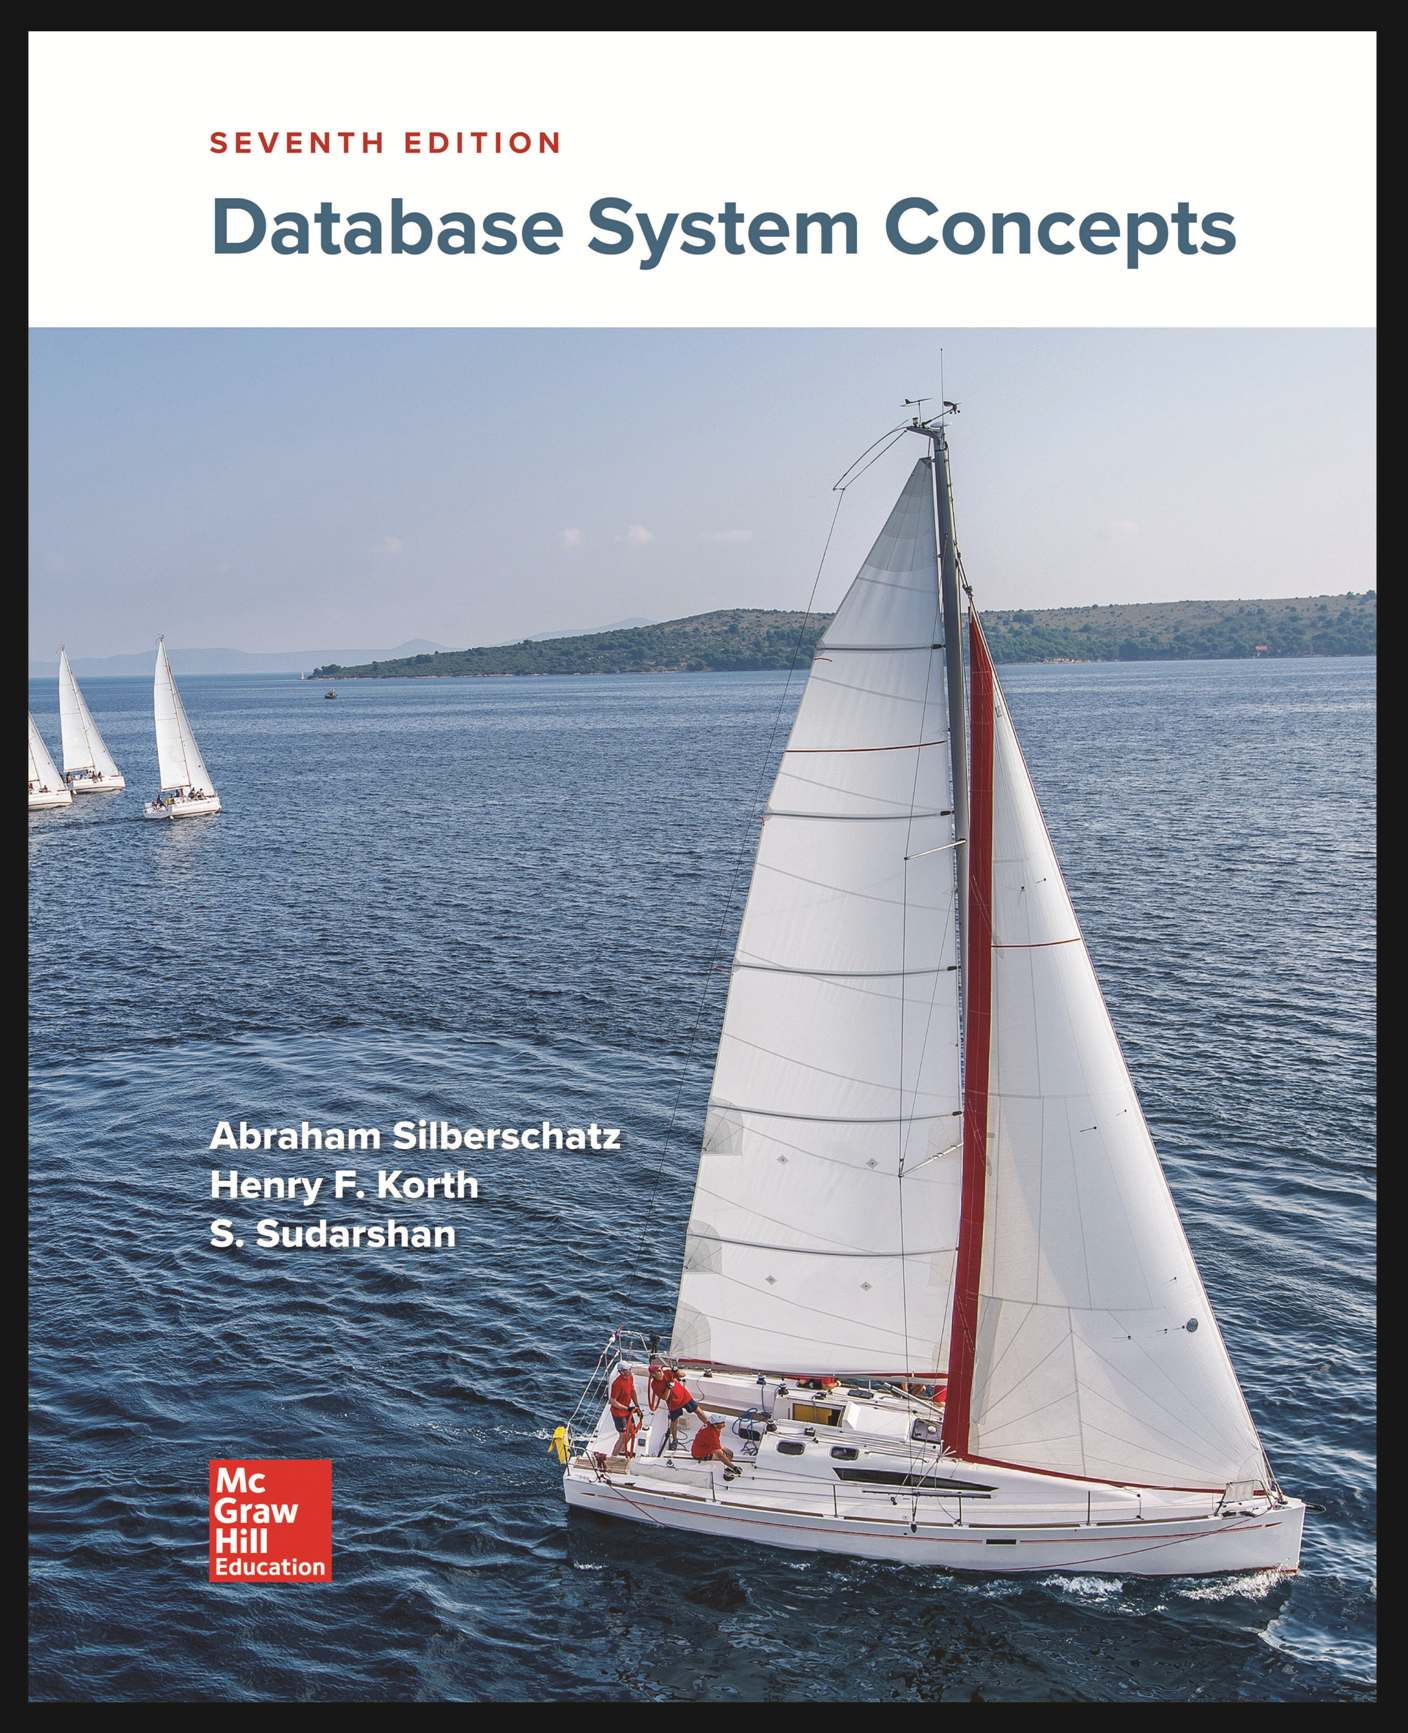
\includegraphics[width=0.5\textwidth]{figures/book_cover.jpg} \\
    \vspace{5mm}
    {
        \tiny
        Content has been extracted from \textit{Database System Concepts}, Seventh Edition, by Silberschatz, Korth and Sudarshan. Mc Graw Hill Education. 2019.\\
        Visit \url{https://db-book.com/}.\\
    }
\end{frame}

\section{Overview of The SQL Query Language}

\begin{frame}{History}
    \begin{itemize}
        \item IBM Sequel language developed as part of System R project at IBM San Jose Research Laboratory.
        \item Renamed Structured Query Language (SQL).
        \item ANSI and ISO standard SQL:
        \begin{itemize}
            \item SQL-86
            \item SQL-89
            \item SQL-92
            \item SQL:1999\footnote{language name became Y2K compliant!.}
            \item SQL:2003
        \end{itemize}
        \item Commercial systems offer most, if not all, SQL-92 features, plus varying feature sets from later standards and special proprietary features.
        \begin{itemize}
            \item Not all examples here may work on your particular system.
        \end{itemize}
    \end{itemize}
\end{frame}

\begin{frame}{SQL Parts}
    \begin{itemize}
        \item DML -- provides the ability to query information from the database and to insert tuples into, delete tuples from, and modify tuples in the database.
        \item Integrity -- the DDL includes commands for specifying integrity constraints.
        \item View definition -- the DDL includes commands for defining views.
    \end{itemize}
\end{frame}

\begin{frame}{SQL Parts}
    \begin{itemize}
        \item Transaction control -- includes commands for specifying the beginning and ending of transactions.
        \item Embedded SQL and dynamic SQL -- define how SQL statements can be embedded within general-purpose programing languages.
        \item Authorization -- includes commands for specifying access rights to relations and views.
    \end{itemize}
\end{frame}

\section{SQL Data Definition}

\begin{frame}{Data Definition Language}
    The SQL data-definition language (DDL) allows the specification of information about relations, including:
    \begin{itemize}
        \item The schema for each relation.
        \item The type of values associated with each attribute.
        \item The integrity constraints.
        \item The set of indices to be maintained for each relation.
        \item Security and authorization information for each relation.
        \item The physical storage structure of each relation on disk.
    \end{itemize}
\end{frame}

\begin{frame}{Domain Types in SQL}
    \begin{itemize}
        \item \texttt{char(n).} Fixed length character string, with user-specified length \texttt{n}.
        \item \texttt{varchar(n).} Variable length character string, with user-specified maximum length \texttt{n}.
        \item \texttt{int.} Integer (a finite subset of integers that is machine-dependent).
        \item \texttt{smallint.} Small integer (a machine-dependent subset of integer domain type).
    \end{itemize}
\end{frame}

\begin{frame}{Domain Types in SQL}
    \begin{itemize}
        \item \texttt{numeric(p, d).} Fixed point number, with user-specified precision of \texttt{p} digits, with \texttt{d} digits to the right of decimal point. (ex., \texttt{numeric(3,1)}, allows 44.5 to be stores exactly, but not 444.5 or 0.32).
        \item \texttt{real, double precision.} Floating point and double-precision floating point numbers, with machine-dependent precision.
        \item \texttt{float(n).} Floating point number, with user-specified precision of at least \texttt{n} digits.
        \item More are covered in Chapter 4.
    \end{itemize}
\end{frame}

\begin{frame}[fragile]{Create Table Construct}
    \begin{itemize}
        \item An SQL relation is defiend using the \texttt{create table} command:
        \begin{lstlisting}[language=SQL]
CREATE TABLE @($r\text{ }($)@
        @($A_1 D_1, A_2 D_2, \ldots, A_n D_n, $)@
        @($(integrity\_constraints_1),$)@
        @($(integrity\_constraints_2),$)@
            @($\vdots$)@
        @($(integrity\_constraints_k)$)@
@($);$)@
        \end{lstlisting}
        \begin{itemize}
            \item $r$ is the name of the relation.
            \item each $A_i$ is an attribute name in the schema of relation $r$.
            \item $D_i$ is the data type of values in the domain of attribute $A_i$.
        \end{itemize}
    \end{itemize}
\end{frame}

\begin{frame}[fragile]{Create Table Construct}
    \begin{exampleblock}{Example:}
    \begin{minted}
    [tabsize=4, obeytabs, frame=lines, framesep=2mm, baselinestretch=1.2, bgcolor=LightGray, fontsize=\footnotesize, linenos]{sql}
    CREATE TABLE instructor (
        ID char(5),
        name varchar(20),
        dept_name varchar(20),
        salary numeric(8,2)
    );
    \end{minted}
    \end{exampleblock}
\end{frame}

\begin{frame}{Integrity Constraints in Create Table}
    \begin{itemize}
        \item Types of integrity constraints:
        \begin{itemize}
            \item \texttt{primary key}$(A_{j_1}, \ldots, A_{j_m})$
            \item \texttt{foreing key}$(A_{k_1}, \ldots, A_{k_n})$
            \item \texttt{not null}
        \end{itemize}
        \item SQL prevents any update to the database that violates an integrity constraint.
    \end{itemize}
\end{frame}

\begin{frame}[fragile]{Integrity Constraints in Create Table}
    \begin{exampleblock}{Example:}
    \begin{minted}
    [tabsize=4, obeytabs, frame=lines, framesep=2mm, baselinestretch=1.2, bgcolor=LightGray, fontsize=\footnotesize, linenos]{sql}
    CREATE TABLE instructor (
        ID          char(5),
        name        varchar(20),
        dept_name   varchar(20),
        salary      numeric(8,2),
        primary key (ID),
        foreign key (dept_name) references deparment
    );
    \end{minted}
    \end{exampleblock}
\end{frame}

\begin{frame}[fragile]{Few more Relation Definitions}
    \begin{exampleblock}{Example:}
    \begin{minted}
    [tabsize=4, obeytabs, frame=lines, framesep=2mm, baselinestretch=1.2, bgcolor=LightGray, fontsize=\footnotesize, linenos]{sql}
    CREATE TABLE student (
        ID          varchar(5),
        name        varchar(20) not null,
        dept_name   varchar(20),
        tot_cred    numeric(3,0),
        primary key (ID),
        foreign key (dept_name) references department
    );
    \end{minted}
    \end{exampleblock}
\end{frame}

\begin{frame}[fragile]{Few more Relation Definitions}
    \begin{exampleblock}{Example:}
    \begin{minted}
    [tabsize=4, obeytabs, frame=lines, framesep=2mm, baselinestretch=1.2, bgcolor=LightGray, fontsize=\footnotesize, linenos]{sql}
    CREATE TABLE takes (
        ID          varchar(5),
        course_id   varchar(8),
        sec_id      varchar(8),
        semester    varchar(6),
        year        numeric(4,0),
        grade       varchar(2),
        primary key (ID, course_id, sec_id, semester, year),
        foreign key (ID) references student,
        foreign key (course_id, sec_id, semester, year)
            references section
    );
    \end{minted}
    \end{exampleblock}
\end{frame}

\begin{frame}[fragile]{And more still}
    \begin{exampleblock}{Example:}
    \begin{minted}
    [tabsize=4, obeytabs, frame=lines, framesep=2mm, baselinestretch=1.2, bgcolor=LightGray, fontsize=\footnotesize, linenos]{sql}
    CREATE TABLE course (
        course_id   varchar(8),
        title       varchar(50),
        dept_name   varchar(20),
        credits     numeric(2,0),
        primary key (course_id),
        foreign key (dept_name) references department
    );
    \end{minted}
    \end{exampleblock}
\end{frame}

\begin{frame}[fragile]{Updates to Tables}
    \begin{itemize}
        \item Insert:
    \end{itemize}
    \begin{minted}
    [tabsize=4, obeytabs, frame=lines, framesep=2mm, baselinestretch=1.2, bgcolor=LightGray, fontsize=\footnotesize]{sql}
        INSERT INTO instructor
            VALUES ('10211','Smith','Biology', 66000);
    \end{minted}
    \begin{itemize}
        \item Delete:
    \end{itemize}
    \begin{minted}
    [tabsize=4, obeytabs, frame=lines, framesep=2mm, baselinestretch=1.2, bgcolor=LightGray, fontsize=\footnotesize]{sql}
        DELETE FROM studentes;
    \end{minted}
    \begin{itemize}
        \item Drop a table:
    \end{itemize}
    \begin{minted}
    [tabsize=4, obeytabs, frame=lines, framesep=2mm, baselinestretch=1.2, bgcolor=LightGray, fontsize=\footnotesize]{sql}
        DROP TABLE r;
    \end{minted}
\end{frame}

\begin{frame}{Updates to Tables}
    \begin{itemize}
        \item Alter:
        \begin{itemize}
            \item alter table $r$ add $A$ $D$:
            \begin{itemize}
                \item where $A$ is the name of the attribute to be added to relation $r$ and $D$ is the domain of $A$.
                \item all existing tuples in the relation are assigned \textit{null} as the value for the new attribute.
            \end{itemize}
            \item alter table $r$ drop $A$:
            \begin{itemize}
                \item where $A$ is the name of an attribute of relation $r$.
                \item dropping of attributes not supported by many databases.
            \end{itemize}
        \end{itemize}
    \end{itemize}
\end{frame}

\section{Basic Query Structure of SQL Queries}

\begin{frame}[fragile]{Basic Query Structure}
    \begin{itemize}
        \item A typical SQL query has the form:
        \begin{lstlisting}[language=SQL]
SELECT
    @($A_1, A_2, \ldots, A_n$)@
FROM
    @($r_1, r_2, \ldots, r_m$)@
WHERE
    @(P)@
        \end{lstlisting}
        \begin{itemize}
            \item $A_i$ represents an attribute.
            \item $r_i$ represents a relation.
            \item $P$ is a predicate.
        \end{itemize}
        \item The result of an SQL is a relation.
    \end{itemize}
\end{frame}

\begin{frame}[fragile]{The SELECT Clause}
    \begin{itemize}
        \item The \texttt{SELECT} clause lists the attributes desired in the result of a query.
        \begin{itemize}
            \item It corresponds to the projection ($\Pi$) operation of the relational algebra.
        \end{itemize}
    \end{itemize}
    \begin{exampleblock}{Example:}
        ``Find the names of all instructors.''
    \end{exampleblock}
    \begin{minted}
    [tabsize=4, obeytabs, frame=lines, framesep=2mm, baselinestretch=1.2, bgcolor=LightGray, fontsize=\footnotesize]{sql}
    SELECT name FROM instructor;
    \end{minted}
\end{frame}

\begin{frame}{The SELECT Clause}
    \begin{alertblock}{Note}
        SQL names are case sensitive (i.e., you may use upper- or lower-case letters.)
        \begin{itemize}
            \item E.g., Name $\equiv$ NAME $\equiv$ name.
            \item Some people use upper case wherever we use bold font.
        \end{itemize}
    \end{alertblock}
\end{frame}

\begin{frame}[fragile]{The SELECT Clause (Cont.)}
    \begin{itemize}
        \item SQL allows duplicates in relations as well as in query results.
        \item To force the elimination of duplicates, insert the keyword \texttt{DISTINCT} after the \texttt{SELECT} clause.
    \end{itemize}
    \begin{exampleblock}{Example:}
        ``Find the deparment names of all instructors, and remove duplicates.''
    \end{exampleblock}
    \begin{minted}
    [tabsize=4, obeytabs, frame=lines, framesep=2mm, baselinestretch=1.2, bgcolor=LightGray, fontsize=\footnotesize]{sql}
    SELECT DISTINCT dept_name FROM instructor;
    \end{minted}
    \vspace{-7mm}
    \begin{itemize}
        \item The keyword \texttt{ALL} specifies that duplicates should not be remove.
    \end{itemize}
    \begin{minted}
    [tabsize=4, obeytabs, frame=lines, framesep=2mm, baselinestretch=1.2, bgcolor=LightGray, fontsize=\footnotesize]{sql}
    SELECT ALL dept_name FROM instructor;
    \end{minted}
\end{frame}

\begin{frame}[fragile]{The SELECT Clause (Cont.)}
    \begin{itemize}
        \item An asterisk ($*$) in the \texttt{SELECT} clause denotes ``all attributes''.
        \begin{minted}
        [tabsize=4, obeytabs, frame=lines, framesep=2mm, baselinestretch=1.2, bgcolor=LightGray, fontsize=\footnotesize]{sql}
        SELECT * FROM instructor;
        \end{minted}
        \item An attribute can be a literal with \texttt{FROM} clause.
        \begin{minted}
        [tabsize=4, obeytabs, frame=lines, framesep=2mm, baselinestretch=1.2, bgcolor=LightGray, fontsize=\footnotesize]{sql}
        SELECT 'A' FROM instructor;
        \end{minted}
        \vspace{-5mm}
        \begin{itemize}
            \item Result is a table with one column and $N$ rows (number of tuples in the $instructor$ table), each row with value ``A''.
        \end{itemize}
    \end{itemize}
\end{frame}

\begin{frame}[fragile]{The SELECT Clause (Cont.)}
    \begin{itemize}
        \item An attribute can be a literal with no \texttt{FROM} clause.
        \begin{minted}
        [tabsize=4, obeytabs, frame=lines, framesep=2mm, baselinestretch=1.2, bgcolor=LightGray, fontsize=\footnotesize]{sql}
        SELECT '42';
        \end{minted}
        \vspace{-5mm}
        \begin{itemize}
            \item Results is a table with one column and a single row with value ``42''.
            \item Can give the column a name using:
            \begin{minted}
            [tabsize=4, obeytabs, frame=lines, framesep=2mm, baselinestretch=1.2, bgcolor=LightGray, fontsize=\footnotesize]{sql}
            SELECT '42' AS foo;
            \end{minted}
        \end{itemize}
    \end{itemize}
\end{frame}

\begin{frame}[fragile]{The SELECT Clause (Cont.)}
    \begin{itemize}
        \item The SELECT clause can contain arithmetic expression involving the operation, $+$, $-$, $*$, and $/$, and operating on constants or attributes of tuples.
        \begin{itemize}
            \item The query:
                \begin{minted}
                [tabsize=4, obeytabs, frame=lines, framesep=2mm, baselinestretch=1.2, bgcolor=LightGray, fontsize=\footnotesize]{sql}
    SELECT ID, name, salary/12 FROM instructor;
                \end{minted}
                would return a relation that is the same as the $instructor$ relation, except that the value of the attribute \texttt{salary} is divided by 12.
            \item Can rename \texttt{``salary/12''} using the \texttt{AS} clause
                \begin{minted}
                [tabsize=4, obeytabs, frame=lines, framesep=2mm, baselinestretch=1.2, bgcolor=LightGray, fontsize=\footnotesize]{sql}
    SELECT ID, name, salary/12 AS monthly_salary
    FROM instructor;
                \end{minted}
        \end{itemize}
    \end{itemize}
\end{frame}

\begin{frame}[fragile]{The WHERE Clause}
    \begin{itemize}
        \item The \texttt{WHERE} clause specifies conditions that the result must satisfy
        \begin{itemize}
            \item Corresponds to the selection ($\sigma$) predicate of the relational algebra.
        \end{itemize}
        \item
        \begin{exampleblock}{Example:}
            ``Find all instructors in Comp. Sci. department.''
        \end{exampleblock}
        \begin{minted}
        [tabsize=4, obeytabs, frame=lines, framesep=2mm, baselinestretch=1.2, bgcolor=LightGray, fontsize=\footnotesize]{sql}
    SELECT name
    FROM instructor
    WHERE dept_name = 'Comp. Sci.';
        \end{minted}
    \end{itemize}
\end{frame}

\begin{frame}[fragile]{The WHERE Clause}
    \begin{itemize}
        \item SQL  allows the use of the logical connectives \textbf{and}, \textbf{or},  and \textbf{not}.
        \item The operands of the logical connectives can be expressions involving the comparison operators $<$, $<=$, $>$, $>=$, $=$, and $<>$.
        \item Comparisons can be applied to results of arithmetic expressions.
            \begin{exampleblock}{Example:}
                ``Find all instructors in Comp. Sci. with salary $>$ 80000.''
            \end{exampleblock}
            \begin{minted}
            [tabsize=4, obeytabs, frame=lines, framesep=2mm, baselinestretch=1.2, bgcolor=LightGray, fontsize=\footnotesize]{sql}
        SELECT name
        FROM instructor
        WHERE dept_name = 'Comp. Sci.' AND salary > 80000;
            \end{minted}
    \end{itemize}
\end{frame}

\begin{frame}[fragile]{The FROM Clause}
    \begin{itemize}
        \item The \texttt{FROM} clause lists the relations involved in the query.
        \begin{itemize}
            \item Corresponds to the Cartesian product ($\times$) operation of the relational algebra.
        \end{itemize}
        \begin{exampleblock}{Example:}
            ``Find the Cartesian producto $instructor \times teaches$.''
        \end{exampleblock}
        \begin{minted}
        [tabsize=4, obeytabs, frame=lines, framesep=2mm, baselinestretch=1.2, bgcolor=LightGray, fontsize=\footnotesize]{sql}
    SELECT *
    FROM instructor, teaches;
        \end{minted}
    \end{itemize}
\end{frame}

\begin{frame}{The FROM Clause}
    \begin{itemize}
        \item[ ]
        \begin{itemize}
            \item generates every possible instructor $–$ teaches pair, with all attributes from both relations.
            \item for common attributes (e.g., \texttt{ID}), the attributes in the resulting table are renamed using the relation name (e.g., \texttt{instructor.ID})
        \end{itemize}
        \item Cartesian product is not very useful directly, but it is useful combined with the \texttt{WHERE} clause condition ($\sigma$ operation in relational algebra).
    \end{itemize}
\end{frame}

\begin{frame}[fragile]{Examples}
    \begin{exampleblock}{}
        ``Find the names of all instructors who have taught some course and the course\_id.''
    \end{exampleblock}\pause

    \begin{minted}
    [tabsize=4, obeytabs, frame=lines, framesep=2mm, baselinestretch=1.2, bgcolor=LightGray, fontsize=\footnotesize, linenos]{sql}
    SELECT
        name, course_id
    FROM
        instructor, teaches
    WHERE
        instructor.ID = teaches.ID;
    \end{minted}
\end{frame}

\begin{frame}[fragile]{Examples}
    \begin{exampleblock}{}
        ``Find the names of all instructors in the Art deparment who have taught some course and the course\_id.''
    \end{exampleblock}\pause

    \begin{minted}
    [tabsize=4, obeytabs, frame=lines, framesep=2mm, baselinestretch=1.2, bgcolor=LightGray, fontsize=\footnotesize, linenos]{sql}
    SELECT
        name, course_id
    FROM
        instructor, teaches
    WHERE
        instructor.ID = teaches.ID AND
        instructor.dept_name = 'Art';
    \end{minted}
\end{frame}

\section{Additional Basic Operations}

\begin{frame}[fragile]{The Rename Operation}
    \begin{itemize}
        \item The SQL allows renaming relations and attributes using the \texttt{AS} clause:
        $$
            old\_name \text{ \texttt{AS} } new\_name
        $$
    \end{itemize}
    \vspace{-8mm}
    \begin{exampleblock}{}
        ``Find the names of all instructors who have a higher salary than some instructor in Comp. Sci. deparment.''
    \end{exampleblock}
    \begin{minted}
    [tabsize=4, obeytabs, frame=lines, framesep=2mm, baselinestretch=1.2, bgcolor=LightGray, fontsize=\footnotesize, linenos]{sql}
    SELECT DISTINCT
        T.name
    FROM
        instructor AS T, instructor AS S
    WHERE
        T.salary > S.salary AND
        S.dept_name = 'Comp. Sci.';
    \end{minted}
\end{frame}

\begin{frame}[fragile]{The Rename Operation}
    \begin{itemize}
        \item keyword \texttt{AS} is optional and may be omitted.
        $$
            instructor \text{ \texttt{AS} } \equiv instructor \text{ } T
        $$
    \end{itemize}
\end{frame}

\begin{frame}{Self Join Example}
    \begin{itemize}
        \item Relation $employee-supervisor$:
            \begin{tabular}{| l | l |}
                \hline
                \textbf{person} & \textbf{supervisor} \\
                \hline
                Bob & Alice \\ \hline
                Mary & Susan \\ \hline
                Alice & David \\ \hline
                David & Mary \\ \hline
            \end{tabular}
        \item Exercises:
        \begin{itemize}
            \item ``Find the supervisor of Bob''
            \item ``Find the supervisor of the supervisor of Bob''
            \item ``Could you find ALL the supervisor (direct and indirect) of Bob?''
        \end{itemize}
    \end{itemize}
\end{frame}

\begin{frame}[fragile]{String Operations}
    \begin{itemize}
        \item SQL includes a string-matching operator for comparisons on character strings.  The operator \texttt{LIKE} uses patterns that are described using two special characters:
        \begin{itemize}
            \item percent (\%) -- The \% character matches any substring.
            \item underscore(\_) -- The \_ character any character.
        \end{itemize}
    \end{itemize}
    \begin{exampleblock}{Example:}
        ``Find the names of all instructors whose name includes the substring `dar'.''
    \end{exampleblock}
\end{frame}

\begin{frame}[fragile]{String Operations}
    \begin{minted}
    [tabsize=4, obeytabs, frame=lines, framesep=2mm, baselinestretch=1.2, bgcolor=LightGray, fontsize=\footnotesize, linenos]{sql}
    SELECT
        name
    FROM
        instructor
    WHERE
        name LIKE '%dar%';
    \end{minted}
    \vspace{-6mm}
    \begin{itemize}
        \item Match the string `100\%'
        \begin{minted}
        [tabsize=4, obeytabs, frame=lines, framesep=2mm, baselinestretch=1.2, bgcolor=LightGray, fontsize=\footnotesize]{sql}
        LIKE '100\%';
        \end{minted}
        in that above we use backslash (\textbackslash) as the escape character.
    \end{itemize}
\end{frame}

\begin{frame}[fragile]{String Operations (Cont.)}
    \begin{itemize}
        \item Patterns are case sensitive.
        \item Pattern matching examples:
        \begin{itemize}
            \item \texttt{`Intro\%'} matches any string beginning with ``Intro''.
            \item `\%Comp\%' matches any string containing ``Comp'' as a substring.
            \item `\_\_\_' matches any string of exactly three characters.
            \item `\_\_\_\%' matches any string of at least three characters.
        \end{itemize}
        \item SQL supports a variety of string operations such as:
        \begin{itemize}
            \item concatenation (using ``$| |$'').
            \item converting from upper to lower case (and viceversa).
            \item finding string length, extracting substrings, etc.
        \end{itemize}
    \end{itemize}
\end{frame}

\begin{frame}[fragile]{Ordering the Display of Tuples}
    \begin{exampleblock}{Example:}
        ``List in alphabetic order the names of all instructors.''
    \end{exampleblock}
    \begin{minted}
    [tabsize=4, obeytabs, frame=lines, framesep=2mm, baselinestretch=1.2, bgcolor=LightGray, fontsize=\footnotesize, linenos]{sql}
        SELECT DISTINCT
            name
        FROM
            instructor
        ORDER BY
            name;
    \end{minted}
\end{frame}

\begin{frame}[fragile]{Ordering the Display of Tuples}
    \begin{itemize}
        \item We may specify \texttt{DESC} for descending order of \texttt{ASC} for ascending order, for each attribute; \texttt{ASC} is the default.
        \begin{minted}
        [tabsize=4, obeytabs, frame=lines, framesep=2mm, baselinestretch=1.2, bgcolor=LightGray, fontsize=\footnotesize]{sql}
            ORDER BY name DESC
        \end{minted}
        \item Can sort in multiple attributes.
        \begin{minted}
        [tabsize=4, obeytabs, frame=lines, framesep=2mm, baselinestretch=1.2, bgcolor=LightGray, fontsize=\footnotesize]{sql}
            ORDER BY dept_name, name
        \end{minted}
    \end{itemize}
\end{frame}

\begin{frame}[fragile]{Where Clause Predicates}
    \begin{itemize}
        \item SQL includes a \texttt{BETWEEN} comparison operator.
    \end{itemize}
    \begin{exampleblock}{Example:}
        ``Find the names of all instructors with salary between \$90000 and \$100000 (that is, $\geq$ \$90000 and $\leq$ \$100000).
    \end{exampleblock}
    \begin{minted}
    [tabsize=4, obeytabs, frame=lines, framesep=2mm, baselinestretch=1.2, bgcolor=LightGray, fontsize=\footnotesize, linenos]{sql}
        SELECT
            name
        FROM
            instructor
        WHERE
            salary BETWEEN 90000 AND 100000;
    \end{minted}
\end{frame}

\begin{frame}[fragile]{Where Clause Predicates (Cont.)}
    \begin{itemize}
        \item Tuple comparison:
    \end{itemize}
    \begin{minted}
    [tabsize=4, obeytabs, frame=lines, framesep=2mm, baselinestretch=1.2, bgcolor=LightGray, fontsize=\footnotesize, linenos]{sql}
    SELECT
        name, course_id
    FROM
        instructor, teaches
    WHERE
        (instructor.ID, dept_name) = (teaches.ID = 'Biology');
    \end{minted}
\end{frame}

\section{Set Operations}

\begin{frame}[fragile]{Set Operations}
    \begin{exampleblock}{ }
        ``Find courses that ran in Fall 2017 or in Spring 2018.''
    \end{exampleblock}
    \begin{minted}
    [tabsize=4, obeytabs, frame=lines, framesep=2mm, baselinestretch=1.2, bgcolor=LightGray, fontsize=\scriptsize, linenos]{sql}
(SELECT course_id FROM section WHERE sem = 'Fall' AND year = 2017)
UNION
(SELECT course_id FROM section WHERE sem = 'Spring' AND year = 2018)
    \end{minted}
    \vspace{-10mm}
    \begin{exampleblock}{ }
        ``Find courses that ran in Fall 2017 and in Spring 2018.''
    \end{exampleblock}
    \begin{minted}
    [tabsize=4, obeytabs, frame=lines, framesep=2mm, baselinestretch=1.2, bgcolor=LightGray, fontsize=\scriptsize, linenos]{sql}
(SELECT course_id FROM section WHERE sem = 'Fall' AND year = 2017)
INTERSECT
(SELECT course_id FROM section WHERE sem = 'Spring' AND year = 2018)
    \end{minted}
\end{frame}

\begin{frame}[fragile]{Set Operations (Cont.)}
    \begin{exampleblock}{ }
        ``Find courses that ran in Fall 2017 but not in Spring 2018.''
    \end{exampleblock}
    \begin{minted}
    [tabsize=4, obeytabs, frame=lines, framesep=2mm, baselinestretch=1.2, bgcolor=LightGray, fontsize=\scriptsize, linenos]{sql}
(SELECT course_id FROM section WHERE sem = 'Fall' AND year = 2017)
EXCEPT
(SELECT course_id FROM section WHERE sem = 'Spring' AND year = 2018)
    \end{minted}
    \begin{itemize}
        \item Set operations \texttt{UNION}, \texttt{INTERSECT}, and \texttt{EXCEPT} automatically eliminate duplicates.
        \item To retain all duplicate use \texttt{UNION ALL}, \texttt{INTERSECT ALL}, and \texttt{EXCEPT ALL}.
    \end{itemize}
\end{frame}

\section{Null Values}

\begin{frame}[fragile]{Null Values}
    \begin{itemize}
        \item It is possible for tuples to have a null value, denoted by \texttt{null}, for some of their attributes.
        \item \texttt{null} signifies an unknown value or that a value does not exist.
        \item The results of any arithmetic expression involving \texttt{null} is \texttt{null}.
        \begin{exampleblock}{Example}
            5 + \texttt{null} returns \texttt{null}.
        \end{exampleblock}
    \end{itemize}
\end{frame}

\begin{frame}[fragile]{Null Values (Cont.)}
    \begin{itemize}
        \item The predicate \texttt{IS NULL} can be used to check for null values.
        \begin{exampleblock}{Example}
            ``Find all instructors whose salary is null.''
        \end{exampleblock}
        \begin{minted}
        [tabsize=4, obeytabs, frame=lines, framesep=2mm, baselinestretch=1.2, bgcolor=LightGray, fontsize=\footnotesize]{sql}
    SELECT name FROM instructor WHERE salary IS NULL
        \end{minted}
        \item The predicate \texttt{IS NOT NULL} succeeds if the value on which it is applied is not null.
    \end{itemize}
\end{frame}

\begin{frame}[fragile]{Null Values (Cont.)}
    \begin{itemize}
        \item SQL treats as \textbf{unknown} the result of any comparison involving a null value (other than predicates \texttt{IS NULL} and \texttt{IS NOT NULL}).
        \begin{itemize}
            \item Example: 5 $<$ \texttt{null} or \texttt{null} $<>$ \texttt{null} or \texttt{null} $=$ \texttt{null}
        \end{itemize}
    \end{itemize}
\end{frame}

\begin{frame}[fragile]{Null Values (Cont.)}
    \begin{itemize}
        \item The predicate in a WHERE clause can involve Boolean operations (\texttt{AND}, \texttt{OR}, \texttt{NOT}); thus the definitions of the Boolean operations need to be extended to deal with the value \textbf{unknown}.
        \begin{itemize}
            \item \texttt{AND}:\\ 
                (\texttt{true} \texttt{AND} \textbf{unknown}) = \textbf{unknown}\\
                (\texttt{false} \texttt{AND} \textbf{unknown}) = \texttt{false}\\
                (\textbf{unknown} \texttt{AND} \textbf{unknown}) = \textbf{unknown}\\
            \item \texttt{OR}:\\ 
                (\textbf{unknown} \texttt{OR} \texttt{true}) = \texttt{true}\\
                (\textbf{unknown} \texttt{OR} \texttt{false}) = \textbf{unknown}\\
                (\textbf{unknown} \texttt{OR} \textbf{unknown}) = \textbf{unknown}\\
        \end{itemize}
        \item Result of \texttt{WHERE} clause predicate is treated as \texttt{false} if it evaluates to \textbf{unknown}.
    \end{itemize}
\end{frame}

\section{Aggregate Functions}

\begin{frame}[fragile]{Aggregate Functions}
    \begin{itemize}
        \item These functions operate on the multiset of values of a column of a relation, and return a value:
        \begin{itemize}
            \item \texttt{AVG}: average value.
            \item \texttt{MIN}: minimum value.
            \item \texttt{MAX}: maximum value.
            \item \texttt{SUM}: sum of values.
            \item \texttt{COUNT}: number of values.
        \end{itemize}
    \end{itemize}
\end{frame}

\begin{frame}[fragile]{Aggregate Functions Examples}
    \begin{exampleblock}{}
     ``Find the average salary of instructors in the Computer Science department.''
    \end{exampleblock}
    \begin{minted}
    [tabsize=4, obeytabs, frame=lines, framesep=2mm, baselinestretch=1.2, bgcolor=LightGray, fontsize=\footnotesize, linenos]{sql}
    SELECT
        AVG(salary)
    FROM
        instructor
    WHERE
        dept_name = 'Comp. Sci.';
    \end{minted}
\end{frame}

\begin{frame}[fragile]{Aggregate Functions Examples}
    \begin{exampleblock}{}
     ``Find the total number of instructors who teach a course in the Spring 2018 semester.''
    \end{exampleblock}
    \begin{minted}
    [tabsize=4, obeytabs, frame=lines, framesep=2mm, baselinestretch=1.2, bgcolor=LightGray, fontsize=\footnotesize, linenos]{sql}
    SELECT
        COUNT(DISTINCT ID)
    FROM
        teaches
    WHERE
        semester = 'Spring' AND year = 2018
    \end{minted}
\end{frame}

\begin{frame}[fragile]{Aggregate Functions Examples}
    \begin{exampleblock}{}
     ``Find the number of tuples in the course relation.''
    \end{exampleblock}
    \begin{minted}
    [tabsize=4, obeytabs, frame=lines, framesep=2mm, baselinestretch=1.2, bgcolor=LightGray, fontsize=\footnotesize, linenos]{sql}
    SELECT 
        COUNT(*)
    FROM
        course;
    \end{minted}
\end{frame}

\begin{frame}[fragile]{Aggregate Functions – Group By}
    ``Find the average salary of instructors in each department.''
    \begin{minted}
    [tabsize=4, obeytabs, frame=lines, framesep=2mm, baselinestretch=1.2, bgcolor=LightGray, fontsize=\footnotesize, linenos]{sql}
    SELECT dept_name, AVG(salary) AS avg_salary
    FROM instructor
    GROUP BY dept_name;
    \end{minted}
    \vspace{-5mm}
    \begin{minipage}{.60\textwidth}
        \centering
        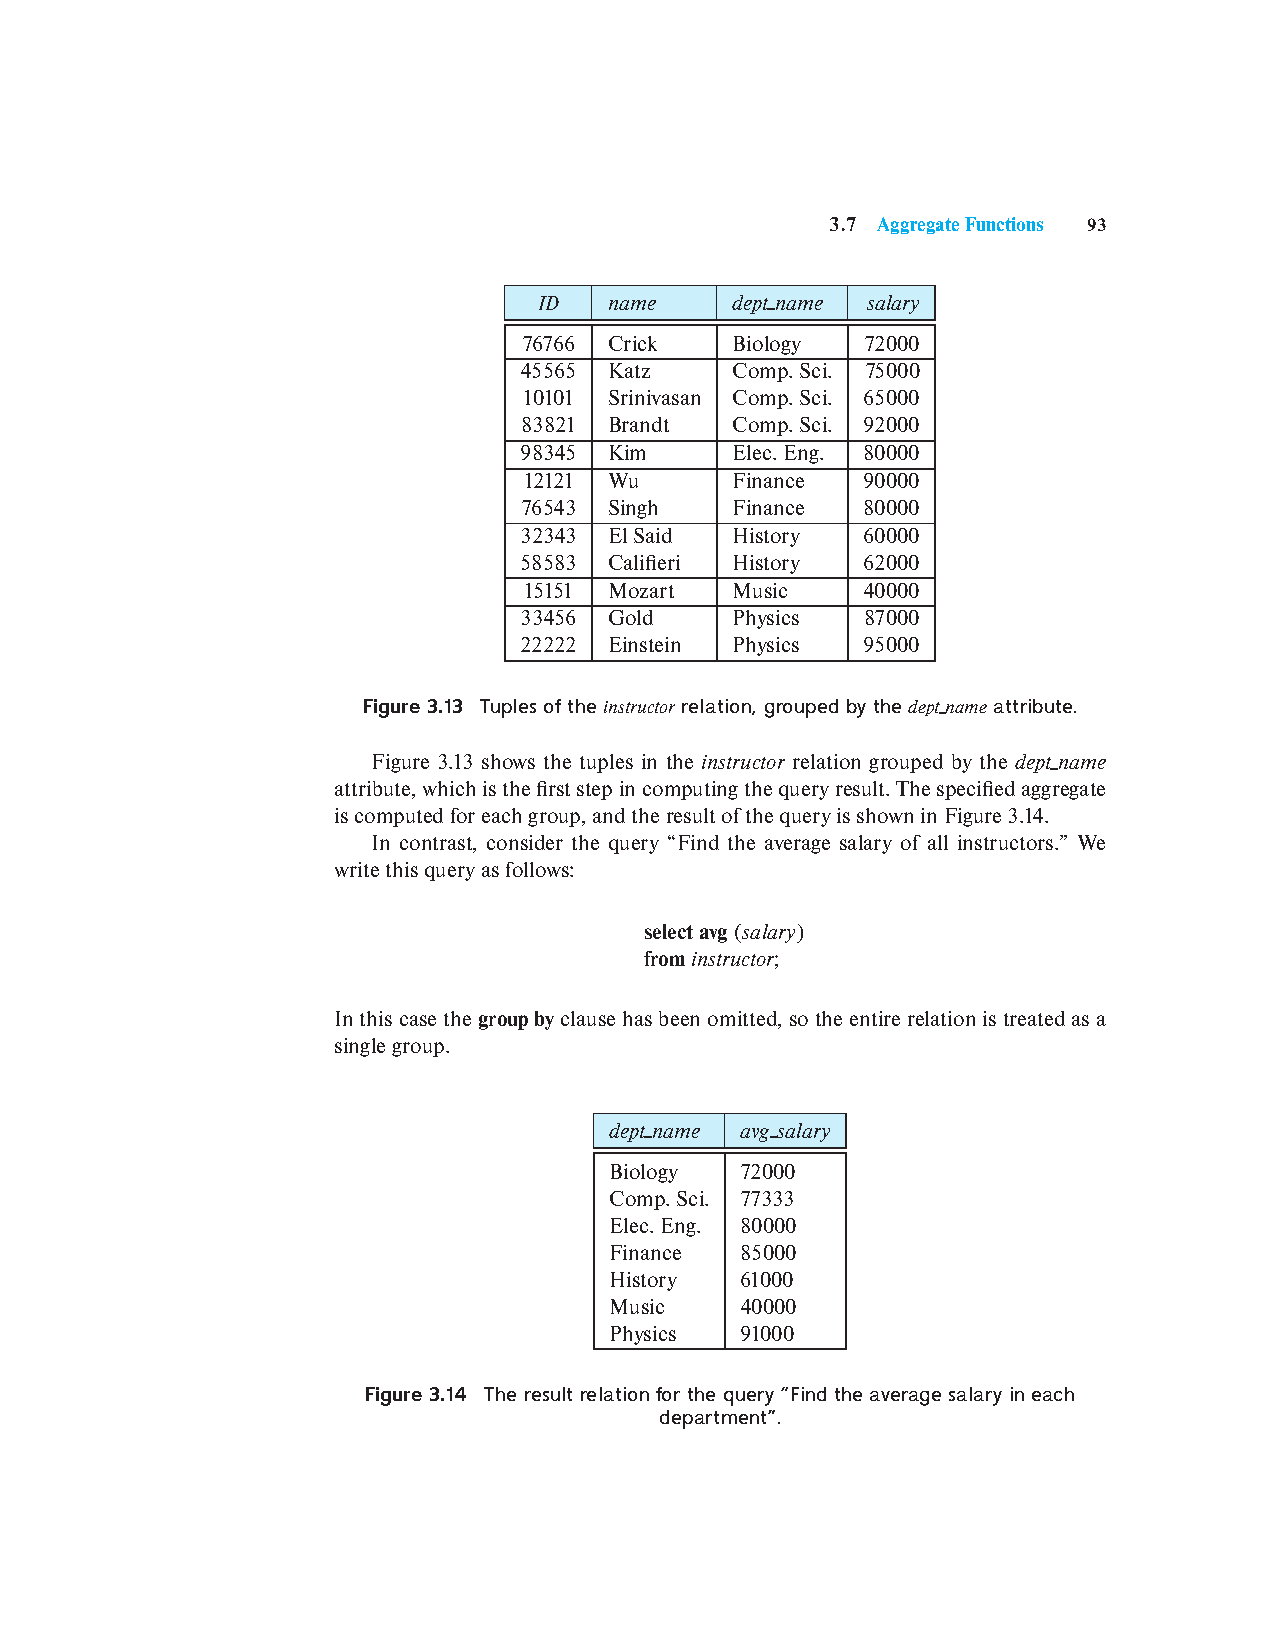
\includegraphics[width=0.9\textwidth, trim={8.5cm 16.5cm 5cm 4.75cm}, clip]{figures/db_agg}    
    \end{minipage}
    \begin{minipage}{.30\textwidth}
        \centering
        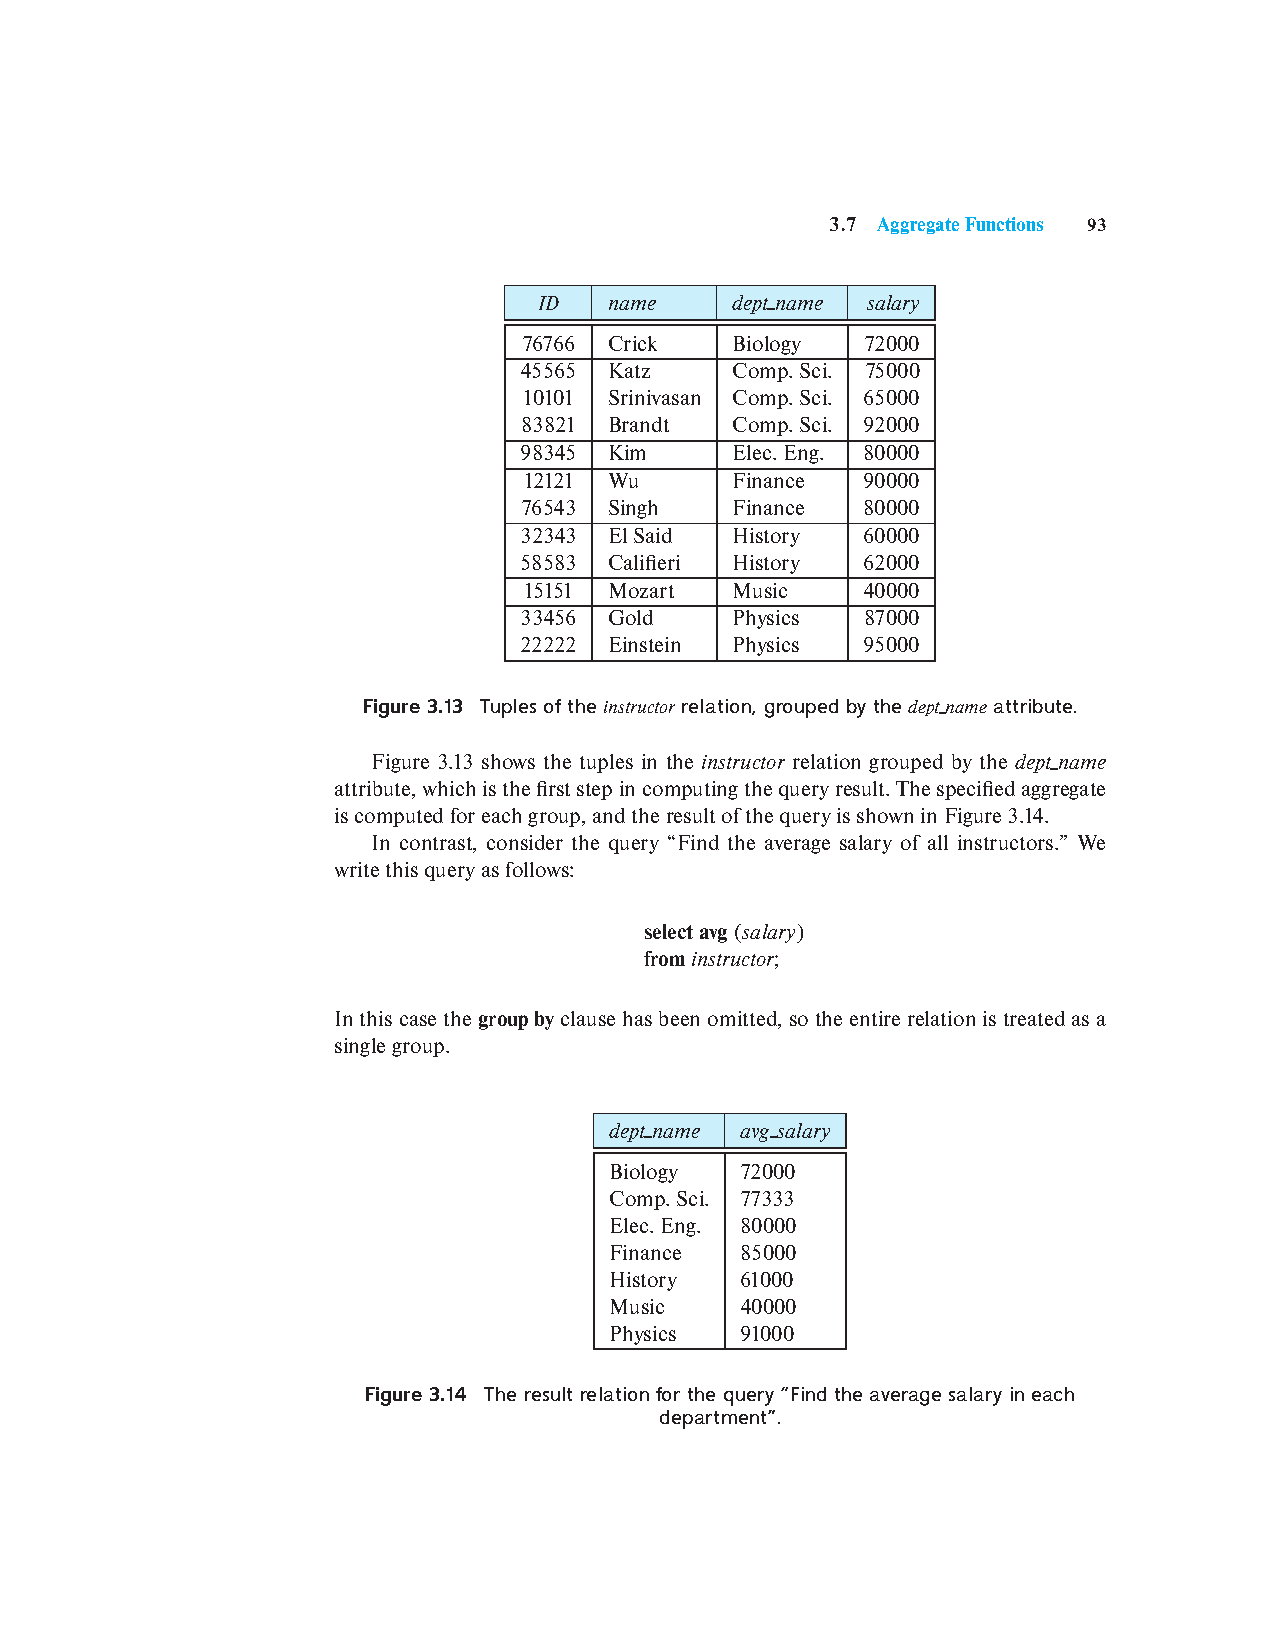
\includegraphics[width=\textwidth, trim={10cm 5cm 7cm 18cm}, clip]{figures/db_agg}    
    \end{minipage}
\end{frame}

\begin{frame}[fragile]{Aggregation (Cont.)}
    \begin{itemize}
        \item Attributes in \texttt{SELECT} clause outside of aggregate functions must appear in \texttt{GROUP BY} list.
    \end{itemize}
    \begin{minted}
    [tabsize=4, obeytabs, frame=lines, framesep=2mm, baselinestretch=1.2, bgcolor=LightGray, fontsize=\footnotesize, linenos]{sql}
    /* erroneous query */
    SELECT 
        dept_name, ID, AVG(salary)
    FROM 
        instructor
    GROUP BY 
        dept_name;
    \end{minted}
\end{frame}

\begin{frame}[fragile]{Aggregate Functions – Having Clause}
    ``Find the names and average salaries of all departments whose average salary is greater than 42000''.
    \begin{minted}
    [tabsize=4, obeytabs, frame=lines, framesep=2mm, baselinestretch=1.2, bgcolor=LightGray, fontsize=\footnotesize, linenos]{sql}
    SELECT dept_name, AVG(salary) as avg_salary
    FROM instructor
    GROUP BY dept_name
    HAVING AVG(salary) > 42000;
    \end{minted}
    \begin{alertblock}{Note:}
        Predicates in the \texttt{HAVING} clause are applied after the formation of groups whereas predicates in the \texttt{WHERE} clause are applied before forming groups.
    \end{alertblock}
\end{frame}

\section{Nested Subqueries}

\begin{frame}[fragile]{Nested Subqueries}
    \begin{itemize}
        \item SQL provides a mechanism for the nesting of subqueries.  A \textbf{subquery} is \texttt{SELECT-FROM-WHERE} expression that is nested within another query.
        \item The nesting can be done in the following SQL query:
        \begin{lstlisting}[language=SQL]
SELECT
    @($A_1, A_2, \ldots, A_n$)@
FROM
    @($r_1, r_2, \ldots, r_m$)@
WHERE
    @($P$)@
        \end{lstlisting}
        as follows:
    \end{itemize}
\end{frame}

\begin{frame}[fragile]{Nested Subqueries}
    \begin{itemize}
        \item[ ]
        \begin{lstlisting}[language=SQL]
SELECT
    @($A_1, A_2, \ldots, A_n$)@
FROM
    @($r_1, r_2, \ldots, r_m$)@
WHERE
    @($P$)@
        \end{lstlisting}
        as follows:
        \begin{itemize}
            \item \textit{From clause}: $r_i$ can be replaced by any valid subquery.
            \item \textit{Where clause}: $P$ can be replaced with an expression of the form:
            $$
                B \text{ } <operation> \text{ } (subquery)
            $$
            $B$ is an attribute and $<operation>$ will be defined later.
            \item \textit{Select clause}: $A_i$ can be replaced be a subquery that generates a single value.
        \end{itemize}
    \end{itemize}
\end{frame}

\begin{frame}[fragile]{Set Membership}
    Find courses offered in Fall 2017 and in Spring 2018.
    \small
    \begin{minted}
    [tabsize=4, obeytabs, frame=lines, framesep=2mm, baselinestretch=1.2, bgcolor=LightGray, fontsize=\footnotesize, linenos]{sql}
    SELECT DISTINCT
        course_id
    FROM
        section
    WHERE
        semester = 'Fall' AND year = 2017 AND
        course_id IN (SELECT
                        course_id
                    FROM
                        section
                    WHERE
                        semester = 'Spring' AND year = 2018
                    );
    \end{minted}
\end{frame}

\begin{frame}[fragile]{Set Membership (Cont.)}
    Find courses offered in Fall 2017 but not in Spring 2018.
    \small
    \begin{minted}
    [tabsize=4, obeytabs, frame=lines, framesep=2mm, baselinestretch=1.2, bgcolor=LightGray, fontsize=\footnotesize, linenos]{sql}
    SELECT DISTINCT
        course_id
    FROM
        section
    WHERE
        semester = 'Fall' AND year = 2017 AND
        course_id NOT IN (SELECT
                        course_id
                    FROM
                        section
                    WHERE
                        semester = 'Spring' AND year = 2018
                    );
    \end{minted}
\end{frame}

\begin{frame}[fragile]{Set Membership (Cont.)}
    Name all instructors whose name is neither ``Mozart'' nor ``Einstein''.
    \begin{minted}
    [tabsize=4, obeytabs, frame=lines, framesep=2mm, baselinestretch=1.2, bgcolor=LightGray, fontsize=\footnotesize, linenos]{sql}
    SELECT DISTINCT
        name
    FROM
        instructor
    WHERE
        name NOT IN ('Mozart', 'Einstein');
    \end{minted}
\end{frame}

\begin{frame}[fragile]{Set Membership (Cont.)}
    Find the total number of (distinct) students who have taken course sections taught by the instructor with ID 10101.
    \begin{minted}
    [tabsize=4, obeytabs, frame=lines, framesep=2mm, baselinestretch=1.2, bgcolor=LightGray, fontsize=\scriptsize, linenos]{sql}
    SELECT
        COUNT(DISTINCT ID)
    FROM
        takes
    WHERE
        (course_id, sec_id, semester, year) IN (
            SELECT
                course_id, sec_id, semester, year
            FROM
                teaches
            WHERE
                teaches.ID = 10101
        );
    \end{minted}
    \vspace{-8mm}
    \begin{alertblock}{\small Note}
        \scriptsize
        Above query can be written in a much simpler manner.  The formulation above is simply to illustrate SQL features.
    \end{alertblock}
\end{frame}

\begin{frame}[fragile]{Set Comparison -- ``some'' Clause}
    Find names of instructors with salary greater than that of some (at least one) instructor in the Biology department.
    \begin{minted}
    [tabsize=4, obeytabs, frame=lines, framesep=2mm, baselinestretch=1.2, bgcolor=LightGray, fontsize=\footnotesize, linenos]{sql}
    SELECT DISTINCT
        T.name
    FROM
        instructor AS T, instructor AS S
    WHERE
        T.salary > S.salary AND
        S.dept_name = 'Biology';
    \end{minted}
\end{frame}

\begin{frame}[fragile]{Set Comparison -- ``some'' Clause (Cont.)}
    Same query using \texttt{$>$ SOME} clause.
    \begin{minted}
    [tabsize=4, obeytabs, frame=lines, framesep=2mm, baselinestretch=1.2, bgcolor=LightGray, fontsize=\footnotesize, linenos]{sql}
    SELECT DISTINCT
        name
    FROM
        instructor
    WHERE
        salary > SOME (
            SELECT
                salary
            FROM
                instructor
            WHERE
                dept_name = 'Biology'
        );
    \end{minted}
\end{frame}

\begin{frame}{Definition of ``some'' Clause}
    $F <comp>$ \texttt{SOME} $r \Leftrightarrow \exists t \in r$ such that $(F <comp> t)$ where $<comp>$ can be: $<$, $\leq$, $>$, $\geq$, $=$, $\neq$.

    \begin{itemize}
        \item[ ]
            \vspace{-5mm}
            \begin{align*}
                \left( 5 < \text{ \texttt{SOME}
                                        \begin{tabular}{|c|}
                                            \hline
                                            0 \\
                                            \hline
                                            5 \\
                                            \hline
                                            6 \\
                                            \hline
                                        \end{tabular} } \right) = true \text{.}
            \end{align*}
            \toRight{\tiny read: 5 $<$ some tuple in the relation.}
        \item[ ]
            \vspace{-5mm}
            \begin{align*}
                \left( 5 < \text{ \texttt{SOME}
                                        \begin{tabular}{|c|}
                                            \hline
                                            0 \\
                                            \hline
                                            5 \\
                                            \hline
                                        \end{tabular} } \right) = false \text{.}
            \end{align*}
        \item[ ]
            \vspace{-5mm}
            \begin{align*}
                \left( 5 = \text{ \texttt{SOME}
                                        \begin{tabular}{|c|}
                                            \hline
                                            0 \\
                                            \hline
                                            5 \\
                                            \hline
                                        \end{tabular} } \right) = true \text{.}
            \end{align*}
        \item[ ]
            \vspace{-5mm}
            \begin{align*}
                \left( 5 \neq \text{ \texttt{SOME}
                                        \begin{tabular}{|c|}
                                            \hline
                                            0 \\
                                            \hline
                                            5 \\
                                            \hline
                                        \end{tabular} } \right) = true \text{.}
            \end{align*}
        \item[Note] ($=$ \texttt{SOME}) $\equiv$ \texttt{IN}.  However, ($\neq$ \texttt{SOME}) $\not\equiv$ \texttt{NOT IN}.
    \end{itemize}
\end{frame}

\begin{frame}[fragile]{Set Comparison -- ``all'' Clause}
    Find the names of all instructors whose salary is greater than the salary of all instructors in the Biology department.
    \begin{minted}
    [tabsize=4, obeytabs, frame=lines, framesep=2mm, baselinestretch=1.2, bgcolor=LightGray, fontsize=\footnotesize, linenos]{sql}
    SELECT
        name
    FROM
        instructor
    WHERE
        salary > ALL (
            SELECT
                salary
            FROM
                instructor
            WHERE
                dept_name = 'Biology'
        );
    \end{minted}
\end{frame}

\begin{frame}{Definition of ``all'' Clause}
    $F <comp>$ \texttt{ALL} $r \Leftrightarrow \exists t \in r (F <comp> t)$.

    \begin{itemize}
        \item[ ]
            \vspace{-5mm}
            \begin{align*}
                \left( 5 < \text{ \texttt{ALL}
                                        \begin{tabular}{|c|}
                                            \hline
                                            0 \\
                                            \hline
                                            5 \\
                                            \hline
                                            6 \\
                                            \hline
                                        \end{tabular} } \right) = false \text{.}
            \end{align*}
        \item[ ]
            \vspace{-5mm}
            \begin{align*}
                \left( 5 < \text{ \texttt{ALL}
                                        \begin{tabular}{|c|}
                                            \hline
                                            6 \\
                                            \hline
                                            10 \\
                                            \hline
                                        \end{tabular} } \right) = true \text{.}
            \end{align*}
        \item[ ]
            \vspace{-5mm}
            \begin{align*}
                \left( 5 = \text{ \texttt{ALL}
                                        \begin{tabular}{|c|}
                                            \hline
                                            4 \\
                                            \hline
                                            5 \\
                                            \hline
                                        \end{tabular} } \right) = false \text{.}
            \end{align*}
        \item[ ]
            \vspace{-5mm}
            \begin{align*}
                \left( 5 \neq \text{ \texttt{ALL}
                                        \begin{tabular}{|c|}
                                            \hline
                                            4 \\
                                            \hline
                                            6 \\
                                            \hline
                                        \end{tabular} } \right) = true \text{.}
            \end{align*}
        \item[Note] ($\neq$ \texttt{ALL}) $\equiv$ \texttt{NOT IN}.  However, ($=$ \texttt{ALL}) $\not\equiv$ \texttt{IN}.
    \end{itemize}
\end{frame}

\begin{frame}{Test for Empty Relations}
     \begin{itemize}
        \item The \texttt{EXISTS} construct returns the value \texttt{true} if the argument subquery is nonempty.
        \item \texttt{EXISTS}
            \LARGE
            $$
                r \Leftrightarrow r \neq \emptyset
            $$
        \item \normalsize \texttt{NOT EXISTS}
            \LARGE
            $$
                r \Leftrightarrow r = \emptyset
            $$
     \end{itemize}
\end{frame}

\begin{frame}[fragile]{Use of ``exists'' Clause}
    \begin{itemize}
        \item Yet another way of specifying the query ``Find all courses taught in both the Fall 2017 semester and in the Spring 2018 semester''.
        \begin{minted}
        [tabsize=4, obeytabs, frame=lines, framesep=2mm, baselinestretch=1.2, bgcolor=LightGray, fontsize=\scriptsize, linenos]{sql}
        SELECT
            course_id
        FROM
            section AS S
        WHERE
            semester = 'Fall' AND year = 2017 AND
            EXISTS (
                SELECT *
                FROM section AS T
                WHERE semester = 'Spring' AND
                    year= 2018 AND
                    S.course_id = T.course_id
            );
        \end{minted}
    \end{itemize}
\end{frame}

\begin{frame}[fragile]{Use of ``exists'' Clause}
    \begin{itemize}
        \item[ ]
        \begin{minted}
        [tabsize=4, obeytabs, frame=lines, framesep=2mm, baselinestretch=1.2, bgcolor=LightGray, fontsize=\tiny, linenos]{sql}
        SELECT
            course_id
        FROM
            section AS S
        WHERE
            semester = 'Fall' AND year = 2017 AND
            EXISTS (
                SELECT *
                FROM section AS T
                WHERE semester = 'Spring' AND
                    year= 2018 AND
                    S.course_id = T.course_id
            );
        \end{minted}
        \item \textbf{Correlation name:} variable \texttt{S} in the outer query.
        \item \textbf{Correlated subquery:} the inner query,
    \end{itemize}
\end{frame}

\begin{frame}[fragile]{Use of ``not exists'' Clause}
    \begin{itemize}
        \item Find all students who have taken all courses offered in the Biology department.
        \begin{minted}
        [tabsize=4, obeytabs, frame=lines, framesep=2mm, baselinestretch=1.2, bgcolor=LightGray, fontsize=\scriptsize, linenos]{sql}
        SELECT DISTINCT
            S.ID, S.name
        FROM
            student AS S
        WHERE
            NOT EXISTS (
                ( SELECT course_id
                    FROM course
                    WHERE dept_name = 'Biology' )
                EXCEPT
                ( SELECT T.course_id
                    FROM takes AS T
                    WHERE S.ID = T.ID )
            );
        \end{minted}
    \end{itemize}
\end{frame}

\begin{frame}[fragile]{Use of ``not exists'' Clause}
    \begin{itemize}
        \item[ ]
        \begin{minted}
        [tabsize=4, obeytabs, frame=lines, framesep=2mm, baselinestretch=1.2, bgcolor=LightGray, fontsize=\tiny, linenos]{sql}
        SELECT DISTINCT
            S.ID, S.name
        FROM
            student AS S
        WHERE
            NOT EXISTS (
                ( SELECT course_id
                    FROM course
                    WHERE dept_name = 'Biology' )
                EXCEPT
                ( SELECT T.course_id
                    FROM takes AS T
                    WHERE S.ID = T.ID )
            );
        \end{minted}
        \vspace{-5mm}
        \begin{itemize}
            \item First nested query lists all courses offered in Biology.
            \item Second nested query lists all courses a particular student took.
        \end{itemize}
        \item \textcolor{red}{Note:} That $X - Y = \emptyset \Leftrightarrow X \subseteq Y$.
        \item \textcolor{red}{Note:} Cannot write this query using \texttt{= ALL} and its variants.
    \end{itemize}
\end{frame}

\begin{frame}[fragile]{Test for Absence of Duplicate Tuples}
    \begin{itemize}
        \item The \texttt{UNIQUE} construct tests whether a subquery has any duplicate tuples in its result.
        \item The \texttt{UNIQUE} construct evaluates to `\texttt{true}' if a given subquery contains no duplicates.
    \end{itemize}
\end{frame}

\begin{frame}[fragile]{Test for Absence of Duplicate Tuples (Cont.)}
    \begin{itemize}
        \item Find all courses that were offered at most once in 2017.
        \begin{minted}
        [tabsize=4, obeytabs, frame=lines, framesep=2mm, baselinestretch=1.2, bgcolor=LightGray, fontsize=\scriptsize, linenos]{sql}
        SELECT
            T.course_id
        FROM
            course AS T
        WHERE
            UNIQUE (
                SELECT
                    R.course_id
                FROM
                    section AS R
                WHERE
                    T.course_id = R.course_id AND
                    R.year = 2017
            );
        \end{minted}
    \end{itemize}
\end{frame}

\begin{frame}[fragile]{Subqueries in the From Clause}
    \begin{itemize}
        \item SQL allows a subquery expression to be used in the \texttt{FROM} clause.
    \end{itemize}
    \begin{exampleblock}{Example:}
        Find the average instructors' salaries of those departments where the average salary is greater than \$42,000.
    \end{exampleblock}
    \begin{minted}
    [tabsize=4, obeytabs, frame=lines, framesep=2mm, baselinestretch=1.2, bgcolor=LightGray, fontsize=\footnotesize, linenos]{sql}
        SELECT
            dept_name, avg_salary
        FROM ( SELECT dept_name, avg (salary) as avg_salary
                FROM instructor
                GROUP BY dept_name )
        WHERE
            avg_salary > 42000;
    \end{minted}
\end{frame}

\begin{frame}[fragile]{Subqueries in the From Clause (Cont.)}
    \begin{itemize}
        \item Nothe that we do not need to use the \texttt{HAVING} clause.
        \item Another way to write the previous query:
    \end{itemize}
    \begin{minted}
    [tabsize=4, obeytabs, frame=lines, framesep=2mm, baselinestretch=1.2, bgcolor=LightGray, fontsize=\footnotesize, linenos]{sql}
        SELECT
            dept_name, avg_salary
        FROM ( SELECT dept_name, avg (salary)
                FROM instructor
                GROUP BY dept_name
            ) AS dept_avg (dept_name, avg_salary)
        WHERE
            avg_salary > 42000;
    \end{minted}
\end{frame}

\begin{frame}[fragile]{WITH Clause}
    \begin{itemize}
        \item The \texttt{WITH} clause provides a way of defining a temporary relation whose definition is available only to the query in which the \texttt{WITH} clause occurs.
    \end{itemize}
    \begin{exampleblock}{Example:}
        Find all departments with the maximum budget.
    \end{exampleblock}
    \begin{minted}
    [tabsize=4, obeytabs, frame=lines, framesep=2mm, baselinestretch=1.2, bgcolor=LightGray, fontsize=\footnotesize, linenos]{sql}
        WITH max_budget (value) AS
        ( SELECT MAX(budget)
          FROM department )
        SELECT
            department.name
        FROM
            department, max_budget
        WHERE
            department.budget = max_budget.value;
    \end{minted}
\end{frame}

\begin{frame}[fragile]{Complex Queries using With Clause}
    \begin{exampleblock}{ }
        Find all departments where the total salary is greater than the average of the total salary at all departments.
    \end{exampleblock}
    \begin{minted}
    [tabsize=4, obeytabs, frame=lines, framesep=2mm, baselinestretch=1.2, bgcolor=LightGray, fontsize=\scriptsize, linenos]{sql}
        WITH dept_total(dept_name, value) AS
        ( SELECT dept_name, sum(salary)
          FROM instructor
          GROUP BY dept_name ),
        dept_total_avg(value) AS
        ( SELECT AVG(value)
          FROM dept_total )
        SELECT
            dept_name
        FROM
            dept_total, dept_total_avg
        WHERE
            dept_total.value > dept_total_avg.value;
    \end{minted}
\end{frame}

\begin{frame}[fragile]{Scalar Subquery}
    \begin{itemize}
        \item Scalar subquery is one which is used where a single value is expected.
    \end{itemize}
    \begin{exampleblock}{Example:}
        List all departments along with the number of instructors in each department.
    \end{exampleblock}
    \begin{minted}
    [tabsize=4, obeytabs, frame=lines, framesep=2mm, baselinestretch=1.2, bgcolor=LightGray, fontsize=\scriptsize, linenos]{sql}
        SELECT
            dept_name,
            ( SELECT count(*)
              FROM instructor
              WHERE department.dept_name = instructor.dept_name )
            AS num_instructors
        FROM
            department;
    \end{minted}
    \vspace{-5mm}
    \begin{itemize}
        \item Runtime error if subquery returns more than one result tuple.
    \end{itemize}
\end{frame}

\section{Modification of the Database}

\begin{frame}{Modification of the Database}
    \begin{itemize}
        \item Deletion of tuples from a given relation.
        \item Insertion of new tuples into a given relation.
        \item Updating of values in some tuples in a given relation.
    \end{itemize}
\end{frame}

\begin{frame}[fragile]{Deletion}
    \vspace{-6mm}
    \begin{exampleblock}{ }
        Delete all instructors.
    \end{exampleblock}
    \begin{minted}
    [tabsize=4, obeytabs, frame=lines, framesep=2mm, baselinestretch=1.2, bgcolor=LightGray, fontsize=\scriptsize]{sql}
        DELETE FROM instructor;
    \end{minted}
    \pause
    \vspace{-12mm}
    \begin{exampleblock}{ }
        Delete all instructors from the Finance department.
    \end{exampleblock}
    \begin{minted}
    [tabsize=4, obeytabs, frame=lines, framesep=2mm, baselinestretch=1.2, bgcolor=LightGray, fontsize=\scriptsize]{sql}
        DELETE FROM instructor
        WHERE dept_name= 'Finance';
    \end{minted}
    \pause
    \vspace{-12mm}
    \begin{exampleblock}{ }
        Delete all tuples in the instructor relation for those instructors associated with a department located in the Watson building.
    \end{exampleblock}
    \begin{minted}
    [tabsize=4, obeytabs, frame=lines, framesep=2mm, baselinestretch=1.2, bgcolor=LightGray, fontsize=\scriptsize]{sql}
        DELETE FROM instructor
        WHERE dept_name IN ( SELECT dept_name
            FROM department
            WHERE building = 'Watson' );
    \end{minted}
\end{frame}

\begin{frame}[fragile]{Deletion (Cont.)}
    \begin{itemize}
        \item Delete all instructors whose salary is less than the average salary of instructors.
            \begin{minted}
            [tabsize=4, obeytabs, frame=lines, framesep=2mm, baselinestretch=1.2, bgcolor=LightGray, fontsize=\footnotesize, linenos]{sql}
        DELETE FROM instructor
        WHERE salary < ( SELECT AVG(salary)
            FROM instructor );
            \end{minted}
    \end{itemize}
    \begin{itemize}
        \item Problem: as we delete tuples from instructor, the average salary changes
        \item Solution used in SQL:
        \begin{enumerate}
            \item First, compute \texttt{AVG(salary)} and find all tuples to delete.
            \item Next, delete all tuples found above (without recomputing average or retesting the tuples).
        \end{enumerate}
    \end{itemize}
\end{frame}

\begin{frame}[fragile]{Insertion}
    \vspace{-6mm}
    \begin{exampleblock}{ }
        Add a new tuple to course.
    \end{exampleblock}
    \begin{minted}
    [tabsize=4, obeytabs, frame=lines, framesep=2mm, baselinestretch=1.2, bgcolor=LightGray, fontsize=\scriptsize]{sql}
    INSERT INTO course
    VALUES('CS-437', 'Database Systems', 'Comp. Sci.', 4);
    \end{minted}
    \pause
    \vspace{-12mm}
    \begin{exampleblock}{ }
        or equivalently.
    \end{exampleblock}
    \begin{minted}
    [tabsize=4, obeytabs, frame=lines, framesep=2mm, baselinestretch=1.2, bgcolor=LightGray, fontsize=\scriptsize]{sql}
    INSERT INTO course (course_id, title, dept_name, credits)
    VALUES('CS-437', 'Database Systems', 'Comp. Sci.', 4);
    \end{minted}
    \pause
    \vspace{-12mm}
    \begin{exampleblock}{ }
        Add a new tuple to student with \texttt{credits} set to \textbf{null}.
    \end{exampleblock}
    \begin{minted}
    [tabsize=4, obeytabs, frame=lines, framesep=2mm, baselinestretch=1.2, bgcolor=LightGray, fontsize=\scriptsize]{sql}
    INSERT INTO student
    VALUES('3003', 'Green', 'Finance', null);
    \end{minted}
\end{frame}

\begin{frame}[fragile]{Insertion (Cont.)}
    Make each student in the Music department who has earned more than 144 credit hours an instructor in the Music department with a salary of \$18,000.
    \begin{minted}
    [tabsize=4, obeytabs, frame=lines, framesep=2mm, baselinestretch=1.2, bgcolor=LightGray, fontsize=\footnotesize, linenos]{sql}
    INSERT INTO instructor
        SELECT ID, name, dept_name, 18000
        FROM student
        WHERE dept_name = 'Music' AND total_cred > 144;
    \end{minted}
\end{frame}

\begin{frame}[fragile]{Insertion (Cont.)}
    The \texttt{SELECT FROM WHERE} statement is evaluated fully before any of its results are inserted into the relation. \\
    Otherwise queries like:
    \begin{minted}
    [tabsize=4, obeytabs, frame=lines, framesep=2mm, baselinestretch=1.2, bgcolor=LightGray, fontsize=\footnotesize]{sql}
    INSERT INTO table1 SELECT * FROM table1;
    \end{minted}
    would cause problem.
\end{frame}

\begin{frame}[fragile]{Updates}
    \vspace{-6mm}
    \begin{exampleblock}{ }
        Give a 5\% salary raise to all instructors.
    \end{exampleblock}
    \vspace{-2mm}
    \begin{minted}
    [tabsize=4, obeytabs, frame=lines, framesep=2mm, baselinestretch=1.2, bgcolor=LightGray, fontsize=\scriptsize]{sql}
    UPDATE instructor
    SET salary = salary * 1.05;
    \end{minted}
    \pause
    \vspace{-13mm}
    \begin{exampleblock}{ }
        Give a 5\% salary raise to those instructors who earn less than 70000.
    \end{exampleblock}
    \vspace{-2mm}
    \begin{minted}
    [tabsize=4, obeytabs, frame=lines, framesep=2mm, baselinestretch=1.2, bgcolor=LightGray, fontsize=\scriptsize]{sql}
    UPDATE instructor
    SET salary = salary * 1.05
    WHERE salary < 70000;
    \end{minted}
    \pause
    \vspace{-13mm}
    \begin{exampleblock}{ }
        Give a 5\% salary raise to instructors whose salary is less than average.
    \end{exampleblock}
    \vspace{-2mm}
    \begin{minted}
    [tabsize=4, obeytabs, frame=lines, framesep=2mm, baselinestretch=1.2, bgcolor=LightGray, fontsize=\scriptsize]{sql}
    UPDATE instructor
    SET salary = salary * 1.05
    WHERE salary < ( SELECT AVG(salary)
        FROM instructor );
    \end{minted}
\end{frame}

\begin{frame}[fragile]{Updates (Cont.)}
    Increase salaries of instructors whose salary is over \$100,000 by 3\%, and all others by a 5\%.
    \begin{itemize}
        \item Write two update statements:
            \begin{minted}
            [tabsize=4, obeytabs, frame=lines, framesep=2mm, baselinestretch=1.2, bgcolor=LightGray, fontsize=\footnotesize, linenos]{sql}
    UPDATE instructor
    SET salary = salary * 1.03
    WHERE salary > 100000;
    UPDATE instructor
    SET salary = salary * 1.05
    WHERE salary <= 100000;
            \end{minted}
        \item The order is important.
        \item Can be done better using the case statement (next slide)...
    \end{itemize}
\end{frame}

\begin{frame}[fragile]{Case Statement for Conditional Updates}
    Same query as before but with case statement
    \begin{minted}
    [tabsize=4, obeytabs, frame=lines, framesep=2mm, baselinestretch=1.2, bgcolor=LightGray, fontsize=\footnotesize, linenos]{sql}
    UPDATE instructor
    SET salary = CASE
        WHEN salary <= 100000 THEN salary * 1.05
        ELSE salary * 1.03
    END
    \end{minted}
\end{frame}

\begin{frame}[fragile]{Updates with Scalar Subqueries}
    Recompute and update \texttt{tot\_creds} value for all students.
    \begin{minted}
    [tabsize=4, obeytabs, frame=lines, framesep=2mm, baselinestretch=1.2, bgcolor=LightGray, fontsize=\footnotesize, linenos]{sql}
    UPDATE student S
    SET tot_cred = ( SELECT SUM(credits)
        FROM takes, course
        WHERE takes.course_id = course.course_id AND
            S.ID = takes.ID AND
            takes.grade <> 'F' AND
            takes.grade IS NOT NULL );
    \end{minted}
\end{frame}

\begin{frame}[fragile]{Updates with Scalar Subqueries (Cont.)}
    \begin{itemize}
        \item Sets \texttt{tot\_creds} to \textbf{null} for students who have not taken any course.
        \item Instead of \texttt{SUM(credits)}, use:
    \end{itemize}
    \begin{minted}
    [tabsize=4, obeytabs, frame=lines, framesep=2mm, baselinestretch=1.2, bgcolor=LightGray, fontsize=\footnotesize, linenos]{sql}
    CASE
    WHEN SUM(credits) IS NOT NULL THEN SUM(credits)
    ELSE 0
    END
    \end{minted}
\end{frame}

\begin{frame}{}
     \centering
     \Huge End of Chapter 3.
\end{frame}

\section*{Takeaways}

% Tim Duncan's Top 5 Fundamental Takeaways of the Today's Class
\begin{frame}{TDT5FTOTTC}
    \centering
    
\includegraphics[width=0.75\textwidth]{figures/tim.png}
\end{frame}

\begin{frame}{Top 5 Fundamental Takeaways}
    \small
    \begin{enumerate} \pause
        \item[5] \textbf{Handling Nulls and Special Cases:} SQL provides special handling for null values (unknown or missing data) through specific predicates (IS NULL, IS NOT NULL). \pause
        \item[4] \textbf{Data Definition Language (DDL) and Integrity Constraints:} SQL's DDL (CREATE TABLE) defines database schemas, data types, and constraints (primary keys, foreign keys, NOT NULL) to ensure data integrity. \pause
        \item[3] \textbf{Database Modifications (CRUD Operations):} SQL supports data manipulation through statements to insert (INSERT), delete (DELETE), and update (UPDATE) database records based on various conditions. \pause
        \item[2] \textbf{Advanced SQL Operations:} SQL includes powerful features like set operations (UNION, INTERSECT, EXCEPT), aggregates (AVG, COUNT, SUM), grouping (GROUP BY, HAVING), and nested subqueries to handle complex queries. \pause
        \item[1] \textbf{SQL Basics and Structure:} SQL is a standardized language used for querying and managing relational databases using commands like SELECT, FROM, and WHERE.
    \end{enumerate}
\end{frame}

% \section*{Takeaways}
% 
% % Tim Duncan's Top 5 Fundamental Takeaways of the Today's Class
% \begin{frame}{TDT5FTOTTC}
%     \centering
%     
\includegraphics[width=0.75\textwidth]{figures/tim.png}
% \end{frame}
% 
% \begin{frame}{Top 5 Fundamental Takeaways}
%     \small
%     \begin{enumerate} \pause
%         \item[5] \textbf{}. \pause
%         \item[4] \textbf{}. \pause
%         \item[3] \textbf{}. \pause
%         \item[2] \textbf{}. \pause
%         \item[1] \textbf{}.
%     \end{enumerate}
% \end{frame}

\begin{frame}{Database System Concepts}
    \centering
    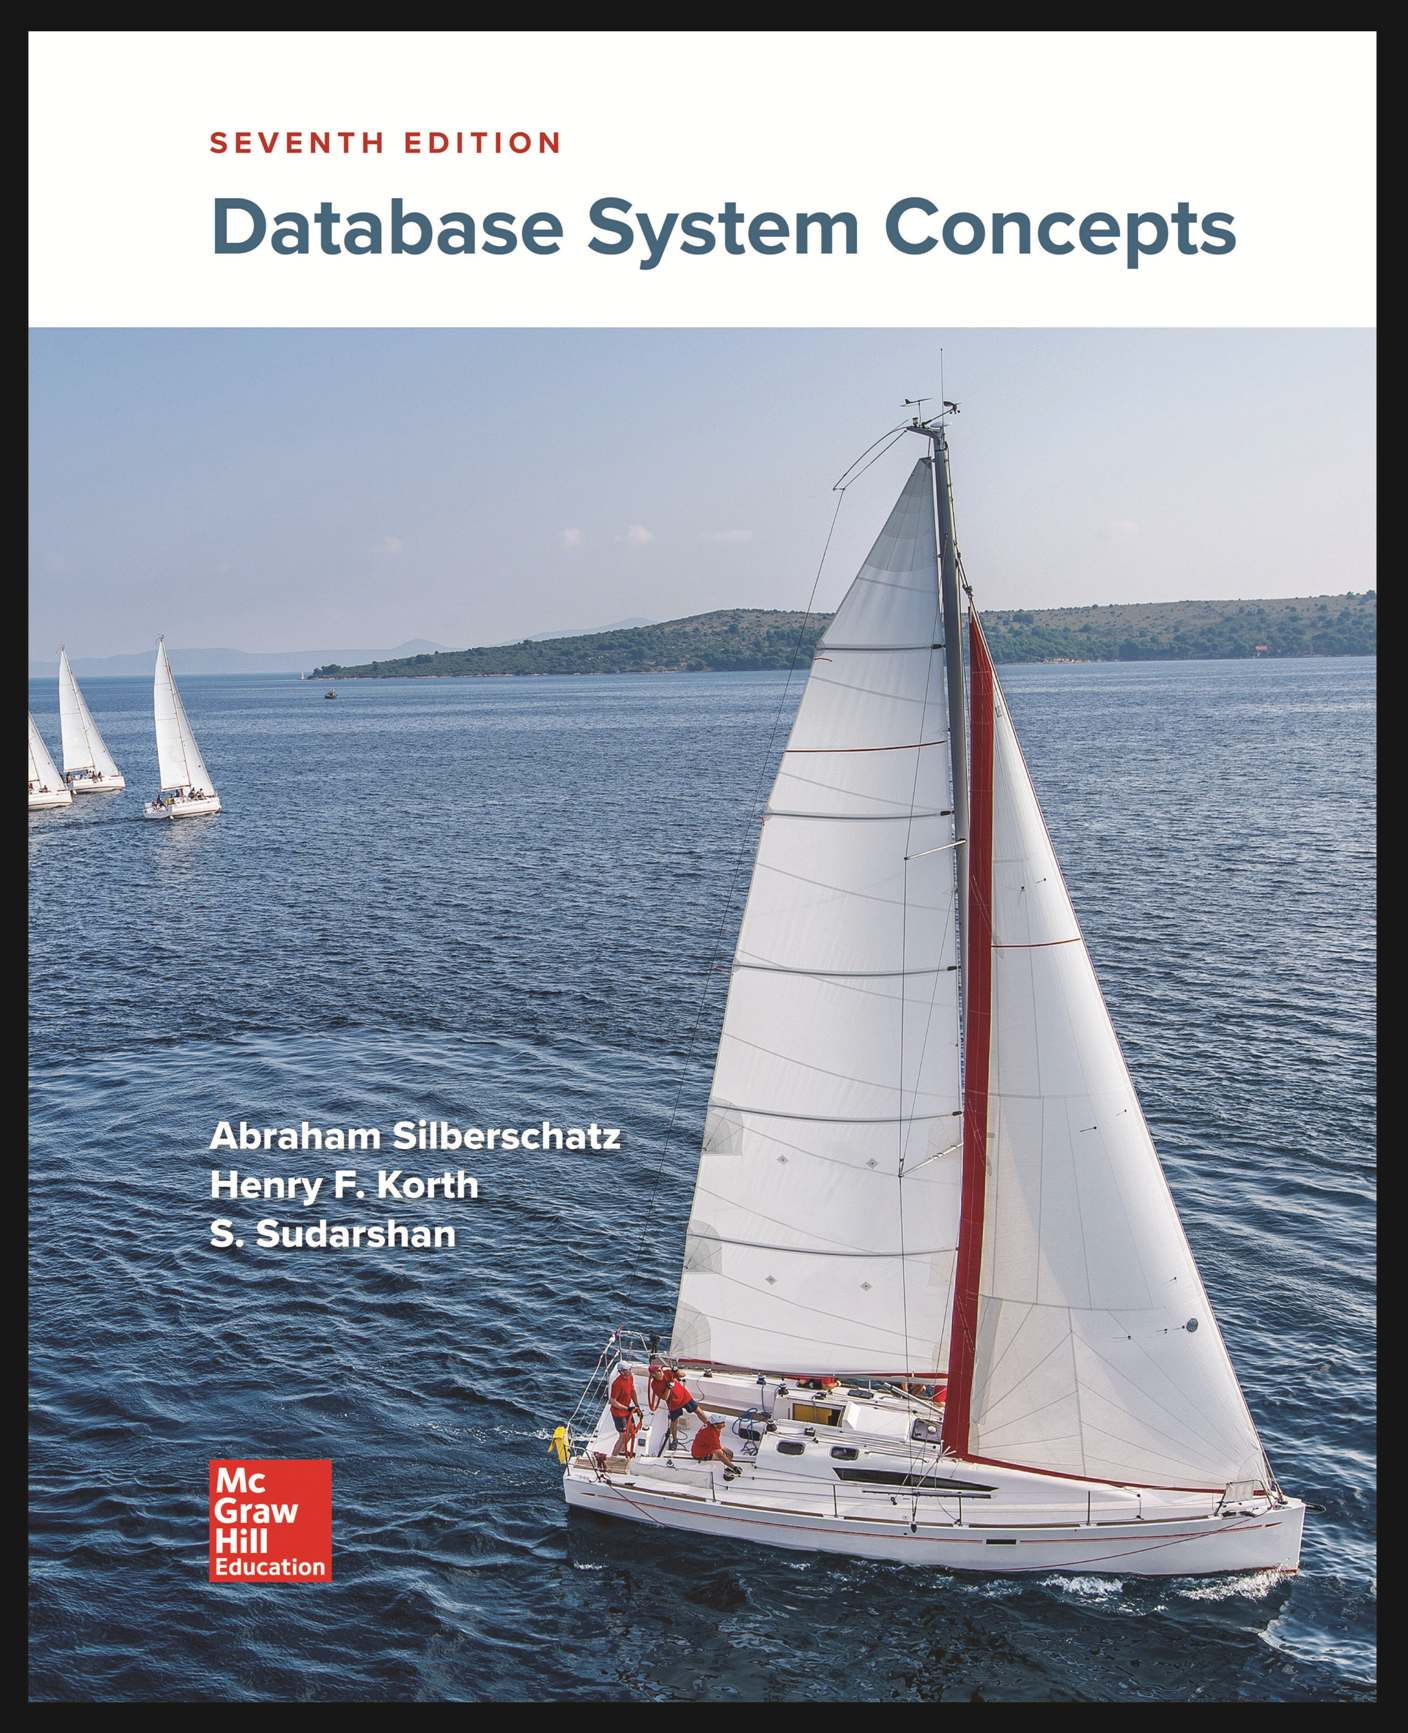
\includegraphics[width=0.5\textwidth]{figures/book_cover.jpg} \\
    \vspace{5mm}
    {
        \tiny
        Content has been extracted from \textit{Database System Concepts}, Seventh Edition, by Silberschatz, Korth and Sudarshan. Mc Graw Hill Education. 2019.\\
        Visit \url{https://db-book.com/}.\\
    }
\end{frame}

\end{document}
